\documentclass[10pt,aspectratio=169,handout]{beamer}

\usepackage[utf8]{inputenc}
\usepackage[ngerman]{babel}
\usepackage{utopia}
\usetheme{Darmstadt}
\usecolortheme{default}
\usepackage{xcolor}
\usepackage{graphicx}
\usepackage{amsmath}
\usepackage{amsthm}
\usepackage{amssymb}
\usepackage{amsfonts}
\usepackage{mathtools}
\usepackage{dsfont}
\usepackage{hyperref}
\usepackage[most]{tcolorbox}
\usepackage{tikz}
\usepackage{adjustbox}
\usepackage{mathrsfs}
\usepackage{minted}
\usetikzlibrary{cd}
\usetikzlibrary{positioning}
\usetikzlibrary{calc}
\usetikzlibrary{arrows.meta}
\setbeamertemplate{theorems}[numbered]
\setbeamertemplate{navigation symbols}{}
\newtranslation[to=ngerman]{Theorem}{Satz}
\def\C{\mathbb{C}}
\def\R{\mathbb{R}}
\def\Q{\mathbb{Q}}
\def\N{\mathbb{N}}
\def\Z{\mathbb{Z}}
\def\cA{\mathcal{A}}
\definecolor{LightGray}{gray}{0.9}


\begin{document}

\title{Principles of Machine Learning: Exercise 5}
\date{11.01.2024}
\author{Alina Pollehn (3197257), Julian Litz (3362592), Manuel Hinz (3334548)\\
    Felix Göhde (3336445), Felix Lehmann (3177181), Caspar Wiswesser (3221493)\\
    Adrian Köring (3347785), Greta Günther (3326765), Linus Mallwitz (3327653)\\
    Niklas Mueller-Goldingen (3363219), Jennifer Kroppen (2783393)}

\begin{frame}
    \maketitle
\end{frame}

\section{Exercise 5.1}

\begin{frame}

    \frametitle{Exercise 4.1: Overview}

    \begin{enumerate}
        \item Goal: Fitting a polynomial to noisy data via polynomial regression
        \item First step: Compute a feature map, where the $i$th column is composed of the powers $x_i^0,\dots,x_i^d$
        \item Second step: Compute the weights: $\hat{w}=[\Phi\Phi^\intercal]^{-1}\Phi y$ using a numerically stable inversion algorithm (i.e. using QR decomposition)
        \item Third step: Compute the fitted model: $\hat{f}(x)=\varphi(x)^\intercal \hat{w}$
    \end{enumerate}

\end{frame}

\begin{frame}
    \frametitle{Results: Plots}

    \begin{minipage}{0.49\textwidth}
        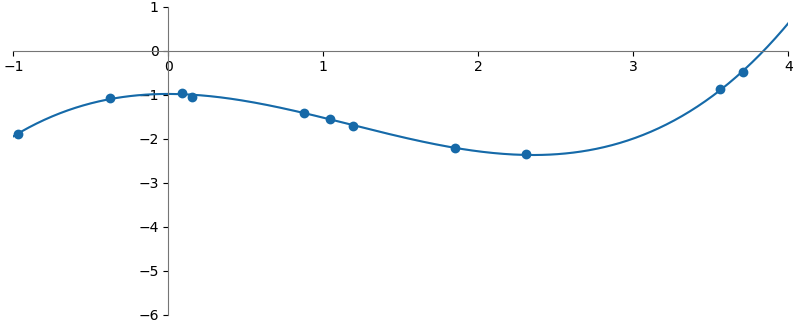
\includegraphics[width=\textwidth]{images/task5-1-2_3.png}
        \captionof{figure}{Polynomial fit for $d=3$}
    \end{minipage}
    \begin{minipage}{0.49\textwidth}
        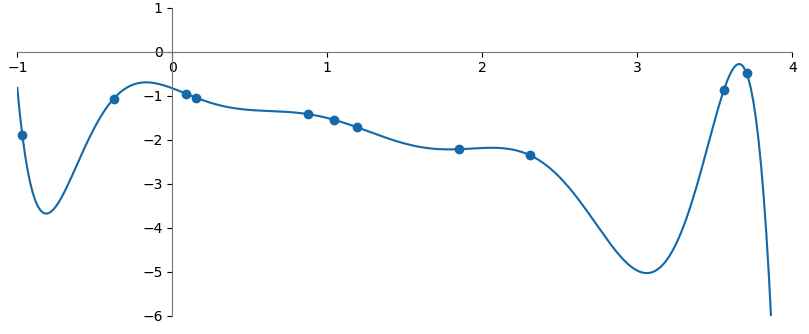
\includegraphics[width=\textwidth]{images/task5-1-2_9.png}
        \captionof{figure}{Polynomial fit for $d=9$}
    \end{minipage}

\end{frame}

\begin{frame}
    \frametitle{Results: Discussion}

    \begin{itemize}
        \item While $d=9$ naturally gives a much better MSE, we not only know (because our data was generated by adding noise to a third degree polynomial), but can clearly see that we are overfitting!
        \item Therefore we would prefer our cubic fit, even if it isn't a perfect
    \end{itemize}

\end{frame}

\begin{frame}
    \frametitle{Adding regularization}

    We now compute the solution to regularized least squares in the same way: $\hat{w}=[\Phi\Phi^\intercal+\lambda I]^{-1}\Phi y$ for different lambda:\newline
    \begin{minipage}{0.32\textwidth}
        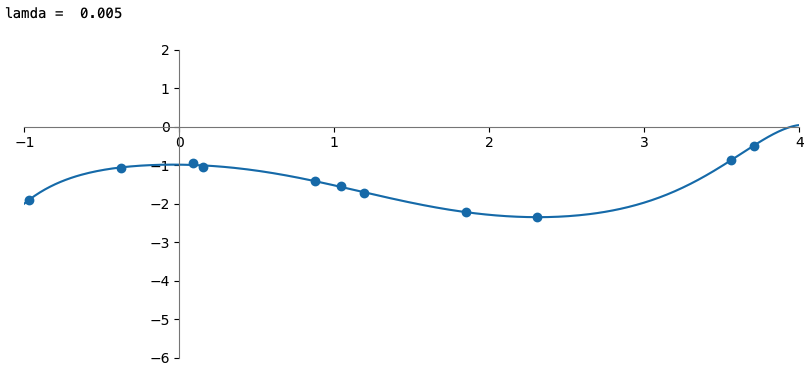
\includegraphics[width=\textwidth]{images/task5-1-3_l0005.png}
        \captionof{figure}{Polynomial fit for $\lambda=0.005$}
    \end{minipage}
    \begin{minipage}{0.32\textwidth}
        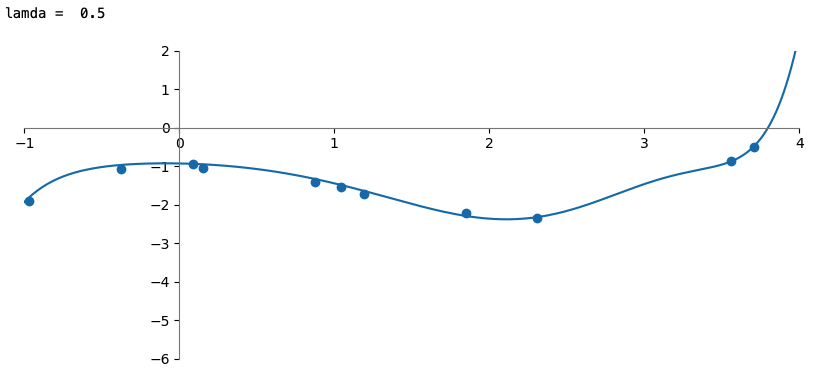
\includegraphics[width=\textwidth]{images/task5-1-3_l05.png}
        \captionof{figure}{Polynomial fit for $\lambda=0.5$}
    \end{minipage}
    \begin{minipage}{0.32\textwidth}
        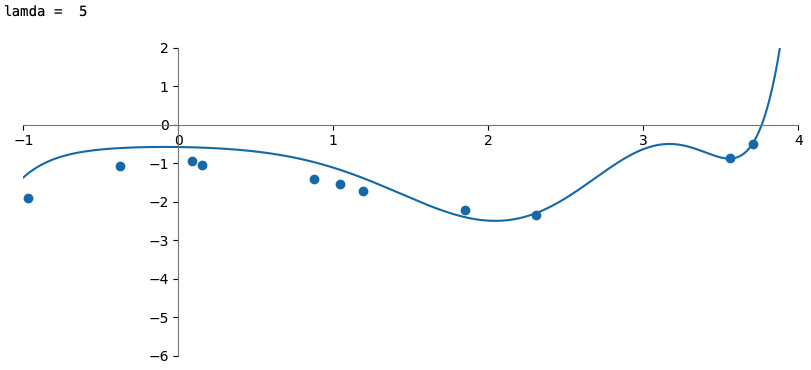
\includegraphics[width=\textwidth]{images/task5-1-3_l5.png}
        \captionof{figure}{Polynomial fit for $\lambda=5$}
    \end{minipage}
\end{frame}

\begin{frame}
    \frametitle{Regularized least squares}

    \begin{itemize}
        \item Great results for smaller $\lambda=0.5,0.005$
        \item $\lambda=5$ gives a worse result, which intuitively makes sense, because we are adding a larger value, decreasing the impact of our gram matrix before inverting!
    \end{itemize}

\end{frame}

\section{Exercise 5.2}

\begin{frame}
    \frametitle{Setting}

    \begin{itemize}
        \item Lecture 07 showed that the dual least squares solution is given by $\hat{w}=\Phi[\Phi\Phi^\intercal]^{-1}y$
        \item After regularization this becomes $\hat{w}=\Phi[\Phi\Phi^\intercal+\lambda I]^{-1}y$
        \item We kernelize the expression $\hat{f}(x)=\phi^\intercal(x)\Phi[\Phi\Phi^\intercal+\lambda I]^{-1}y$ to get \[\hat{f}(x)=k(x)^\intercal[K+\lambda I]^{-1}y\]
        \item Good choices for the model parameters where given: $\lambda=0.5,b=1,d=3$
    \end{itemize}

\end{frame}


\begin{frame}
    \frametitle{Results}

    \begin{minipage}{0.49\textwidth}
        \begin{itemize}
            \item $b$ tranlates the result,
            \item $d$ is the degree of the polynomial, therefore influencing the shape of our model in the usual ways
            \item This, similarly to the previous task, leads to better results for $d=9$, again because of the regularization 
        \end{itemize}
    \end{minipage}
    \begin{minipage}{0.49\textwidth}
        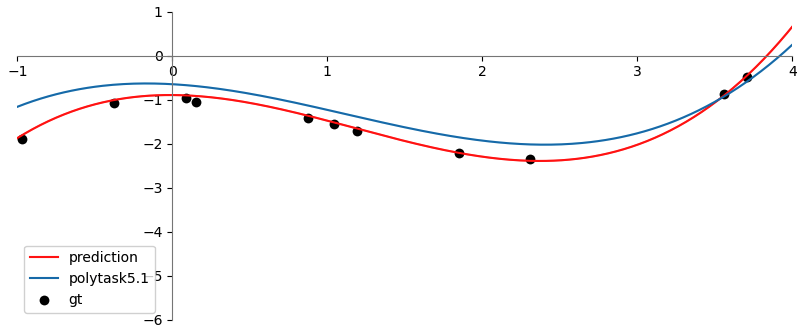
\includegraphics[width=\textwidth]{images/task5-2.png}
        \captionof{figure}{Polynomial fit for the given parameters}
    \end{minipage}

\end{frame}

\section{Exercise 5.3}

\begin{frame}
    \frametitle{Least squares SVMs for regression}

    \begin{itemize}
        \item Adding to the lecture we can use SVMs for regression as well
        \item We want to build a least squares SVM regression model \[\hat{f}(x)=\varphi(x)^\intercal \Phi\hat{\lambda}+\hat{b}\]
        \item Where \[
            \begin{bmatrix}
                \hat{\lambda}\\
                \hat{b}
            \end{bmatrix}=\begin{bmatrix}
                \Phi^\intercal\Phi + \frac{1}{C}I & 1\\
                1^\intercal & 0
            \end{bmatrix}\begin{bmatrix}
                y\\0
            \end{bmatrix}    
        \]
        \item Which can easily be kernelized: \[
            \begin{bmatrix}
                \hat{\lambda}\\
                \hat{b}
            \end{bmatrix}=\begin{bmatrix}
                K + \frac{1}{C}I & 1\\
                1^\intercal & 0
            \end{bmatrix}\begin{bmatrix}
                y\\0
            \end{bmatrix}       
        \] and \[\hat{f}(x)=k(x)^\intercal\hat{\lambda}+\hat{b}\]
    \end{itemize}

\end{frame}

\begin{frame}
    \frametitle{}

    \begin{minipage}{0.49\textwidth}
        \begin{itemize}
            \item Good results for a wider range of parameters (keeping the $d$ fixed)
            \item Results differ more when changing the degree $d$
        \end{itemize}
    \end{minipage}
    \begin{minipage}{0.49\textwidth}
        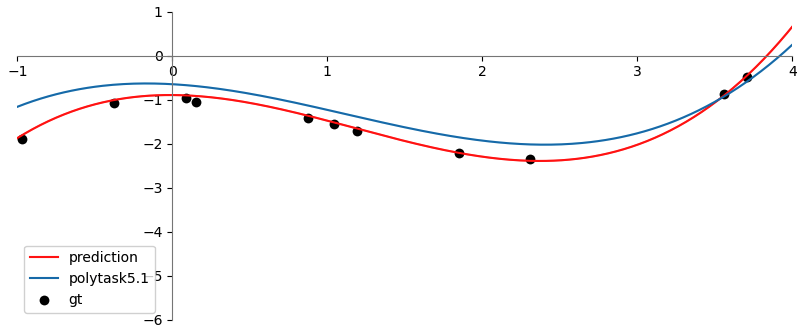
\includegraphics[width=\textwidth]{images/task5-2.png}
        \captionof{figure}{Polynomial fit for the given parameters}
    \end{minipage}

\end{frame}

\begin{frame}
    \frametitle{Other degrees}

    \begin{minipage}{0.49\textwidth}
        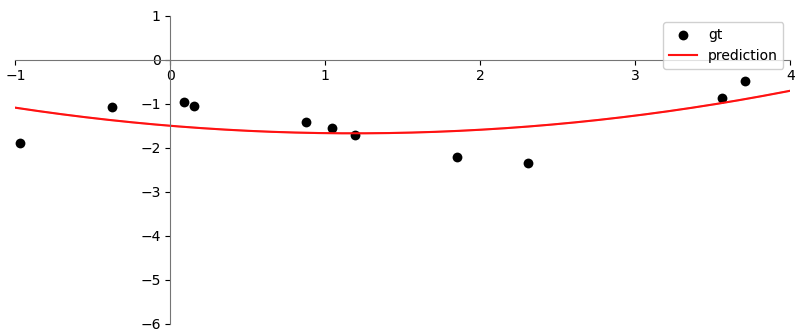
\includegraphics[width=\textwidth]{images/task5-3-d2.png}
        \captionof{figure}{Polynomial fit for the given parameters $d=2$}
    \end{minipage}
    \begin{minipage}{0.49\textwidth}
        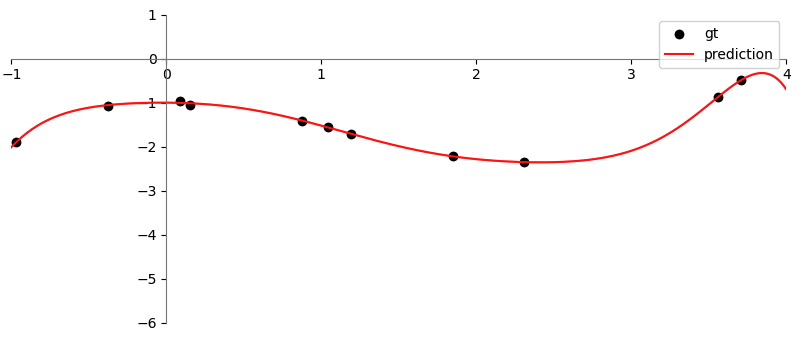
\includegraphics[width=\textwidth]{images/task5-3-d9.png}
        \captionof{figure}{Polynomial fit for the given parameters $d=9$}
    \end{minipage}

\end{frame}

\section{Exercise 5.5}

\begin{frame}
    \frametitle{Minimum enclosing balls}

    \begin{itemize}
        \item We already saw how to compute the minimal enclosing ball for a given dataset in lecture 08:
        \begin{itemize}
            \item Using Frank-Wolfe solve \[\argmin_{\mu} \mu^\intercal X^\intercal X\mu-\mu^\intercal z\]
            \item where $X$ denotes the dataset $X=[x_1,\dots,x_n]\in\mathbb{R}^{m\times n}$ and $z=\text{diag}[X^\intercal X]$
            \item under the constraints $1^\intercal\mu=1$ and $\mu\geq 0$
        \end{itemize}
        \item given $\hat{\mu}$ we can than either compute the radius and the center of the ball 
        \[\hat{c}=X\hat{\mu}\text{  and  } \hat{r}=\sqrt{\hat{\mu^\intercal}z-\hat{\mu}^\intercal X^\intercal X\hat{\mu}}\]
        \item which leads to a function \[\chi_B(x)=\Vert x-\hat{c}\Vert^2 -\hat{r}^2\] which is negative for $x\notin B\cup\partial B$!
        \item we can also rewrite \[\chi_B(x)=x^\intercal x-2x^\intercal X \hat{\mu}+\hat{\mu}^\intercal X^\intercal X \hat{\mu}-\hat{\mu}^\intercal z+\hat{\mu}^\intercal X^\intercal X\hat{\mu}\]
    \end{itemize}

\end{frame}

\begin{frame}
    \frametitle{Result and Frank-Wolfe-Implementation}
    \begin{minipage}{0.49\textwidth}
        \inputminted[bgcolor=LightGray,fontsize=\small]{python}{code/frank_wolfe.py}
    \end{minipage}
    \begin{minipage}{0.49\textwidth}
        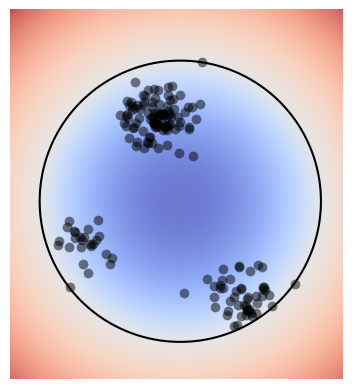
\includegraphics[width=\textwidth]{images/task5-5-2.png}
        \captionof{figure}{$\chi_B(x)$}
    \end{minipage}
\end{frame}

\begin{frame}
    \frametitle{\textbf{Kernel} minimum enclosing balls}

    \begin{itemize}
        \item Using our second formulation \[\chi_B(x)=x^\intercal x-2x^\intercal X \hat{\mu}+\hat{\mu}^\intercal X^\intercal X \hat{\mu}-\hat{\mu}^\intercal z+\hat{\mu}^\intercal X^\intercal X+\hat{\mu}\]
            we can kernalize everything:
        \item We get:\[\chi_B(x)=K(x,x)-2\kappa^\intercal\hat{\mu}-\hat{\mu}^\intercal k+2\hat{\mu}^\intercal K \hat{\mu}\]
        \item where $K(x,x)=\exp(0)=1\in\R$ and  $k=1\in\R^n$, because $k_j=K(x_j,x_j)=\exp(0)=1$.
        \item Using a Gaussian kernel: \[k(u,v)=\exp(-\frac{1}{2\sigma^2}\Vert u-v\Vert^2)\] and the following Frank-Wolfe-Algorithm:
    \end{itemize}

\end{frame}

\begin{frame}
    \frametitle{Frank-Wolfe-Algorithm for kernel minimum enclosing balls}

    \begin{minipage}{0.49\textwidth}
        \begin{itemize}
            \item Solving the minimization problem problem
            \[\begin{aligned}
                &\argmin_{\mu} \mu^\intercal K \mu-\mu^\intercal k\\=&\argmin_{\mu} \mu^\intercal K \mu-\mu^\intercal 1
            \end{aligned}\]
            \item under the constraints $1^\intercal\mu=1$ and $\mu\geq 0$
        \end{itemize}
    \end{minipage}
    \begin{minipage}{0.49\textwidth}
        \inputminted[bgcolor=LightGray,fontsize=\small]{python}{code/frank_wolfe2.py}
    \end{minipage}

\end{frame}

\begin{frame}
    \begin{minipage}[t]{0.45\textwidth}
        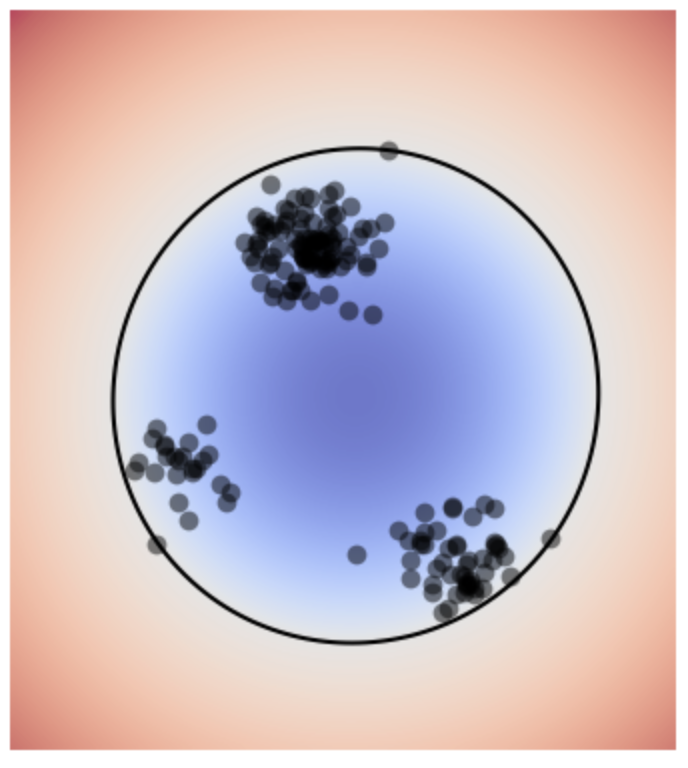
\includegraphics[width=\textwidth]{images/task-5-5-2-4.png}
        \captionof{figure}{$\sigma=4$}
    \end{minipage}
    \begin{minipage}[t]{0.45\textwidth}
        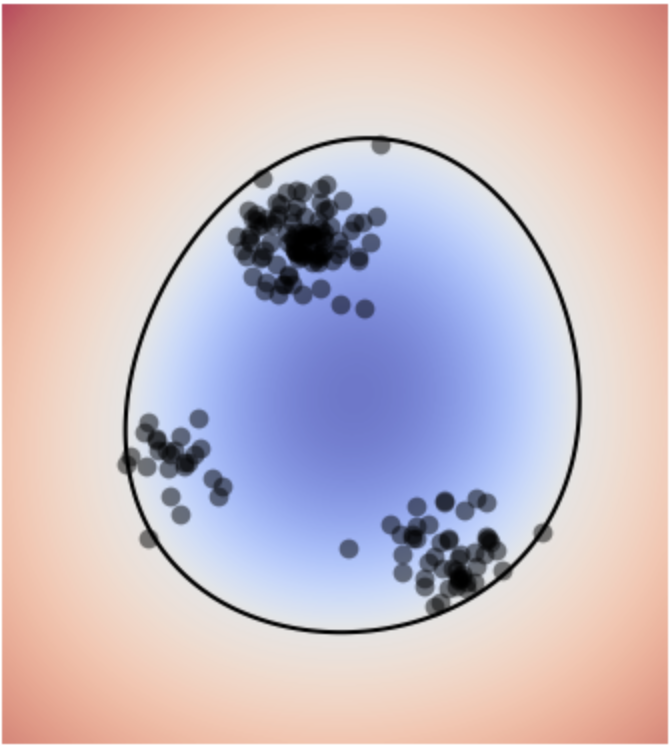
\includegraphics[width=\textwidth]{images/task-5-5-2-2.png}
        \captionof{figure}{$\sigma=2$}
    \end{minipage}
\end{frame}

\begin{frame}
    \begin{minipage}[t]{0.45\textwidth}
        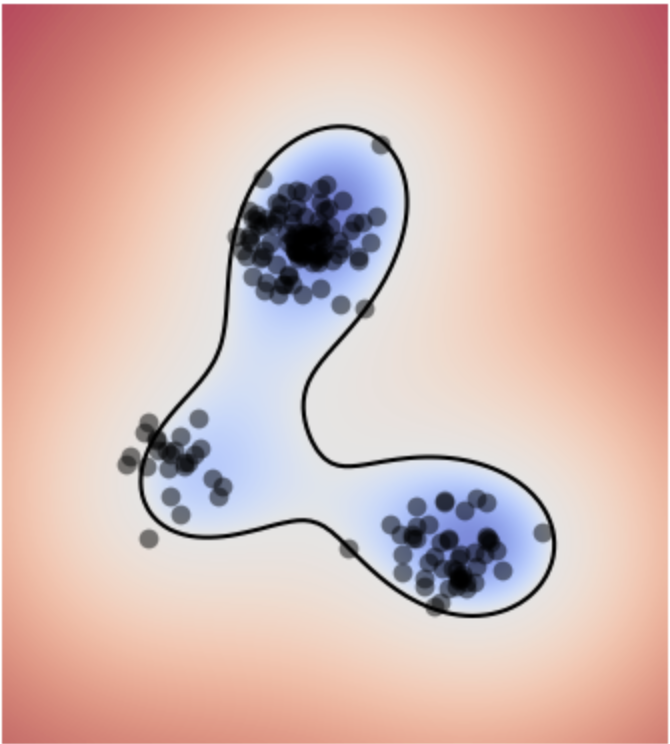
\includegraphics[width=\textwidth]{images/task-5-5-2-1.png}
        \captionof{figure}{$\sigma=1$}
    \end{minipage}
    \begin{minipage}[t]{0.45\textwidth}
        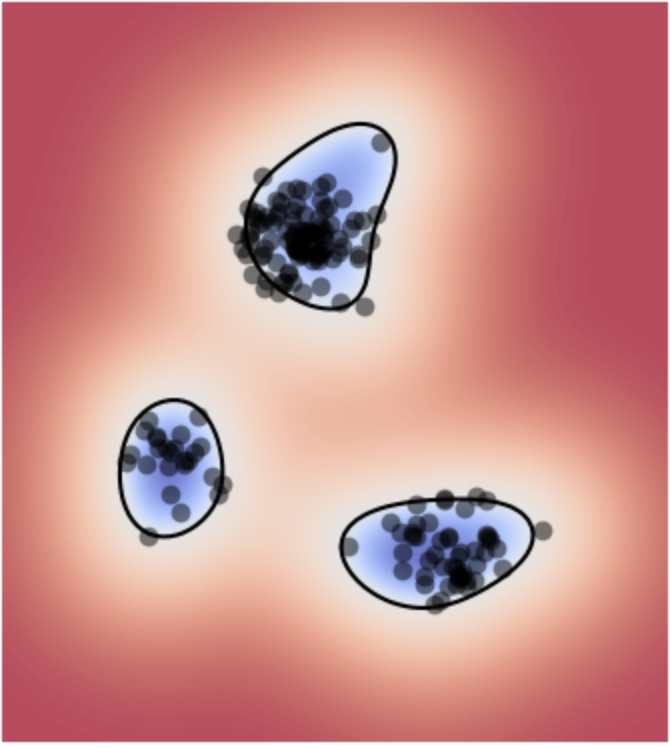
\includegraphics[width=\textwidth]{images/task-5-5-2-05.png}
        \captionof{figure}{$\sigma=0.5$}
    \end{minipage}
\end{frame}

\end{document}
